\documentclass[a4paper,12pt]{report}
\usepackage[english]{babel}
\usepackage{graphicx}
\usepackage{placeins}
\usepackage{hyperref}
\usepackage{supertabular}

\title{CLAM Documentation \\ \small version 0.5-pre-alpha}
\author{Maarten van Gompel \\ Induction of Linguistic Knowledge Research Group \\ Tilburg University }


\newenvironment{devnotes}
{\newpage
\begin{center}
    \begin{tabular}[h!]{|p{0.8\textwidth}|}
    \hline
    {\bf Development Notes}\\\hline}
{   \\\hline
    \end{tabular}
\end{center}}


\begin{document}

\maketitle
\tableofcontents

\chapter{Introduction} 

The Computational Linguistics Application Mediator (CLAM) allows you to quickly and transparently transform your Natural Language Processing application into a \emph{RESTful} webservice, with which automated clients can communicate, but which at the same time also acts as a modern webapplication with which human end-users can interact. CLAM takes a description of your system and wraps itself around the system, allowing clients or users to upload input files to your application, start your application with specific parameters of their choice, and download and view the output of the application. Whilst the application runs, users can monitor its status.

CLAM is set up in a universal fashion, making it flexible enough to be wrapped around a wide range of computational linguistic applications. These applications are treated as a black box, of which only the parameters, input formats and output formats need to be described. The applications themselves need not be network aware in any way, nor aware of CLAM, and the handling and validation of input can be taken care of by CLAM.

CLAM is entirely written in Python and is available as open-source under the GNU Public License (v3), it is set up in a modular fashion and as such is easily extendable. It offers a rich API for writing clients and wrapper scripts.

The kind of applications that CLAM is intended for are Natural Language Processing applications, usually of a kind that do some processing on a text corpus. This corpus or smaller text can be uploaded by the user, or may be pre-installed for the webservice. The NLP application is usually expected to produce a certain output, which is subsequently made available through the webservice for viewing and downloading.

The CLAM webservice is a RESTful webservice, meaning it uses the HTTP verbs GET, POST, PUT and DELETE to manipulate resources and returns responses using the HTTP response codes. The principal resource in CLAM is called a \emph{project}. Various users can maintain various projects, each representing one specific run of the system, with particular input data, output data and a set of configured parameters.

In addition to using HTTP Error Codes for error responses, the webservice responds in the CLAM XML format, an associated XSL stylesheet can directly transform this to xhtml in the user's browser, thus providing a perfect standalone web application for humand end-users. 

CLAM comes with a large number of features, the most notable ones are summarised below:

\begin{itemize}
\item \textbf{RESTful webservice} - \emph{CLAM is a fully RESTful webservice}
\item \textbf{Webapplication} - \emph{CLAM is also a modern ``web 2.0'' web application, heavily relying on technologies such as XSLT and AJAX}
\item \textbf{Extensible} - \emph{Due to the clean and modular setup, CLAM is quite extensible}
\item \textbf{Client and Data API} - \emph{A rich Python API for writing CLAM Clients and system wrappers}
\item \textbf{Authentication} - \emph{A user-based authentication mechanism through HTTP Digest is provided}
\item \textbf{Metadata and provenance data} - \emph{There is extensive support for metadata and provenance data}
\item \textbf{Automatic converters} - \emph{Automatic converters enable conversion from an auxiliary format to the desired input format, and conversion from the produce output format to an auxiliary output format}
\item \textbf{Viewers} - \emph{Viewers enable web-based visualisation for a particular format. CLAM supports both built-in python-based viewers as well as external viewers in the form of external (non-CLAM) webservices.}
\end{itemize}

This documentation is split into two parts: a chapter for service providers, people who want to build a CLAM Webservice around their tool, and a chapter for service clients, users wanting to write automated clients to communicate with the aforemented webservice.

\begin{devnotes}
Note that at this stage, CLAM is still under heavy development. As such, this documentation is not complete yet, but is also a work in progress.
\end{devnotes}


\chapter{Documentation for Service Providers}

\section{Technical details}

CLAM is written in Python 2.5, and is built on the webpy framework. It can run stand-alone thanks to the built-in cherrypy webserver. So no additional webserver is needed to test your service. In production environments, it is however strongly recommended that CLAM is integrated into a real webserver, supported are: Apache, nginx or lighthttpd, though others may work too.

 Note that the software is designed for UNIX systems only!

\subsection{Installation}

The following software is required to run CLAM. These will be available in any modern Linux or BSD distribution:

\begin{itemize}
\item python 2.5 (or a higher 2.x version)
\item python-webpy, version 0.33 or higher
\item python-lxml, version 2 or higher
%\item python-libxslt1
%\item python-django
\end{itemize}

For development and testing, each CLAM webservice can run standalone on any TCP port of your choice (make sure the port is open in your firewall) using the built-in webserver. For production environments, it is strongly recommended you plug CLAM into a more advanced webserver (Apache, nginx, lighttpd). 

To install CLAM, simply uncompress the clam software archive in any desired target location. The following files may be of particular interest:

\begin{itemize}
\item \texttt{clamservice.py} -- This is the webservice itself, the command to be invoked to start it.
\item \texttt{config/} -- This directory contains service configuration files. Place you service configuration here.
\item \texttt{config/defaults.py} -- This is a default configuration template which you can copy to make your own service configuration.
\item \texttt{common/} -- Common Python modules for CLAM
\item \texttt{common/parameters.py} -- Parameter-type definitions
\item \texttt{common/format.py} -- Format-type definitions
\item \texttt{common/data.py} -- CLAM Data API
\item \texttt{common/client.py} -- CLAM Client API
\item \texttt{static/style.css} -- The styling for visualisation
\end{itemize}

Starting the service in standalone mode is done by simply launching clamservice.py with the name of your service configuration (test in the example below). This standalone mode is intended primarily for development purposes and not recommended for production use.

\texttt{\$ ./clamservice.py clam.config.test}

Setting up the service to be used with an already existing webserver, requires some additional work. This is explained below for Apache and nginx:

\subsection{Using CLAM with Apache 2}

In order to run CLAM in Apache, you have to install and configure several files. We will be using WSGI, an interface between Apache and Python. Follow the instructions:

\begin{enumerate}
\item Install \texttt{mod\_wsgi} for Apache 2, if not already present on the system. In Debian and Ubuntu this is available as a package named \texttt{libapache2-mod-wsgi}.
\item Next we need to write a simple WSGI-script, which is a Python script that will be invoked by the webserver. Copy \texttt{clam/config/example.wsgi} to something like  \texttt{clam/config/yourservice.wsgi} and adapt the script. If CLAM is not installed in a standard location where Python can find it, make sure to explicitly specify its parent directory according to the instructions in the example.
\item Configure your service configuration file as explained in Section~\ref{sec:serviceconfig}. Take special note of Subsection~\label{sec:sadmin} where you are instructed to configure the hostname, port and optionally a URL prefix to use if the service isn't assigned a virtualhost of its own.
\item Configure Apache to let it know about WSGI and your service. I assume the reader is acquianted with basic Apache configuration and will only elaborate on the specifics for CLAM. Adapt and add the following to any of your sites in \texttt{/etc/apache2/sites-enabled} (or optionally directly in \texttt{httpd.conf}), within any \texttt{VirtualHost} context. Here it is assumed you configured your service configuration file with \texttt{URLPREFIX} set to \emph{``yourservice''}.

\begin{verbatim}
 WSGIScriptAlias /yourservice /path/to/clam/config/yourservice.wsgi/
 WSGIDaemonProcess yourservice user=proycon group=users \
     home=/path/to/clam threads=15 maximum-requests=10000
 WSGIProcessGroup yourservice

 Alias /yourservice/static /path/to/clam/static/
 <Directory /path/to/clam/static/>
    Order deny,allow
    Allow from all
 </Directory>
\end{verbatim}

The WSGIDaemonProcess directive goes on online, but was wrapped here for presentational purpouses. Needless to say, all paths need to be adapted according to your setup and the configuration can be extended further as desired, with for example extra authentication or more restrictive access. 

\item Restart Apache
\end{enumerate}

Note that we run WSGI in Daemon mode. For the specific options to the WSGIDaemonProcess directive you can check \url{http://code.google.com/p/modwsgi/wiki/ConfigurationDirectives\#WSGIDaemonProcess}, important settings are the user and group the daemon will run as, the home directory it will run in. The number of threads, processes and maximum-requests can also be configured to optimise performance and system resources according to your needs.


\subsection{Using CLAM with nginx}

With nginx (version 0.8 or above), CLAM can be set up over WSGI or FastCGI. With Apache we already explored a WSGI option above, so we will now take a look at FastCGI:

\begin{enumerate}
\item Nginx misses a mime-type we need. Add the following line to \texttt{/etc/nginx/mime.types}:
\begin{verbatim}
  text/xsl                              xsl;
\end{verbatim}

\item Configure your service configuration file as explained in Section~\ref{sec:serviceconfig}. Take special note of Subsection~\label{sec:sadmin} where you are instructed to configure the hostname, port and optionally a URL prefix to use if the service isn't assigned a virtualhost of its own.

\item Make a script \texttt{start\_yourservice.sh} which will start the daemon for FastCGI. Change \texttt{UID} and \texttt{GID} with user ID/group ID you intend to use. Note that the IP and port can be set to anything you like, as long as you use the same consistently throughout the configuration.
\begin{verbatim}
 #!/bin/bash
 spawn-fcgi -u UID -g GID -d /path/to/clam \
   -a 127.0.0.1 -p 9002 -- /path/to/clam/clamservice.py
\end{verbatim}

\item Make a script \texttt{stop\_yourservice.sh} as a convenient shortcut to stop the service again:
\begin{verbatim}
 #!/bin/bash
 kill `pgrep -f "python /path/to/clam/clamservice.py"`
\end{verbatim}

\item Add and adapt the following configuration to a server in \texttt{/etc/nginx/sites-enabled}. Note that in this example, we assume that \texttt{URLPREFIX} in the service configuration file is set to an empty string (or not set at all), effectively exposing CLAM at the root of the server. You may if course configure a \texttt{URLPREFIX} when desired, take care to update the below \texttt{location} and directives accordingly then:
\begin{verbatim}
 root /path/to/clam;

 location / {
    fastcgi_param REQUEST_METHOD $request_method;
    fastcgi_param QUERY_STRING $query_string;
    fastcgi_param CONTENT_TYPE $content_type;
    fastcgi_param CONTENT_LENGTH $content_length;
    fastcgi_param GATEWAY_INTERFACE CGI/1.1;
    fastcgi_param SERVER_SOFTWARE nginx/$nginx_version;
    fastcgi_param REMOTE_ADDR $remote_addr;
    fastcgi_param REMOTE_PORT $remote_port;
    fastcgi_param SERVER_ADDR $server_addr;
    fastcgi_param SERVER_PORT $server_port;
    fastcgi_param SERVER_NAME $server_name;
    fastcgi_param SERVER_PROTOCOL $server_protocol;
    fastcgi_param SCRIPT_FILENAME $fastcgi_script_name;
    fastcgi_param PATH_INFO $fastcgi_script_name;
    fastcgi_pass 127.0.0.1:9002;
 }

 location /static/ {
    root /path/to/clam;
    if (-f $request_filename) {
       rewrite ^/static/(.*)$  /static/$1 break;
    }
 }
\end{verbatim}
\item Launch \texttt{start\_yourservice.sh}  and (re)start nginx.
\end{enumerate}


\subsection{Using CLAM with other webservers}

You are not limited to using either Apache with WSGI or nginx with FastCGI, multiple options are possible, despite the fact we tested only these two. It should also be possible to get CLAM working on other unix based webservers, such as for example lighttpd. Although we have no CLAM-specific instructions, you may find instructions for WebPy, the framework CLAM uses, at \url{http://webpy.org/}, and can adapt these to CLAM.

\section{Architecture}

CLAM has a layered architecture, with at the core the NLP application(s) you want to turn into a webservice. The application itself can remain totally untouched and unaware of CLAM. The scheme in Figure~\ref{fig:arch} illustrates the various layers:

\begin{figure}[h]
\begin{center}
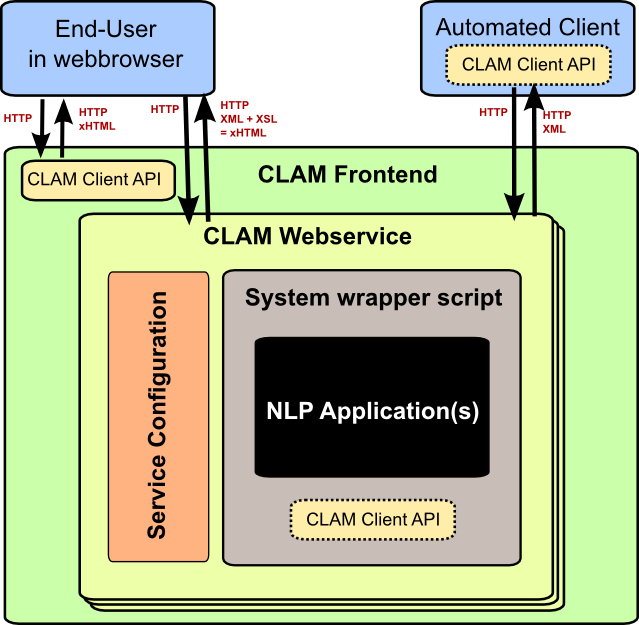
\includegraphics[width=130.0mm]{architecture.png}
\end{center}
\caption{The CLAM Architecture}
\label{fig:arch} 
\end{figure}

The workflow interface layer is not provided nor necessary, but shows a possible use-case.

A CLAM webservice needs the following three components from the service developer:

\begin{enumerate}
\item A service configuration file
\item A wrapper script for your NLP application
\item An NLP application
\end{enumerate}

The wrapper script is not strictly mandatory if the NLP application can be directly invoked by CLAM. However, for more complex applications, writing a wrapper script is strongly recommended, as it offers more flexibility and better integration, and allows you to keep the actual NLP application unmodified. The wrapper scripts can be seen as the ``glue'' between CLAM and your application, taking care of any translation steps.


\section{Service configuration}
\label{sec:serviceconfig}

The service configuration consists of a description of your NLP application, or rather, a description of the system wrapper script that surrounds it. It specifies what parameters the system can take, and what input and output formats are expected under what circumstances. The service configuration is itself a Python script, but knowledge of Python is not essential to be able to make your own service configurations. 

The server configuration files reside in the \texttt{config/} directory. Making a new webservice starts with copying the sample \texttt{defaults.py} and editing your copy. When reading this section, it may help your understanding to inspect this file alongside.

One of the first things to configure is the root path (\texttt{ROOT}). All projects will be confined to the \texttt{projects/} directory within this root path, each project having its own subdirectory. When your NLP application or wrapper script is launched, the current working directory will be set to this project directory. Pre-installed corpora should be put in the \texttt{corpora/} directory. The \texttt{ROOT} will be automatically created upon the first run.


\subsection{Server Administration}
\label{sec:sadmin}

The hostname and port of the webserver can be configured in the service configuration file. Note that the hostname has to match exactly with what the end-users will use, an attempt will be made to detect this automatically if no hostname is specified. A mismatch in the name you define and the hostname the user uses, may result in unexpected behaviour\footnote{Most likely, the XSLT stylesheet will refuse to build the web application interface}. CLAM comes with a built-in webserver, which will be used when it's invoked directly from the command-line\footnote{unless FastCGI mode is enabled}.

When CLAM runs in an existing webserver without its own virtual host, it is often configured at a different URL rather than the webserver root. In this case the value of \texttt{URLPREFIX} should be configured accordingly.

\subsection{Users}

Being a RESTful webservice, user authentication proceeds over HTTP itself. CLAM implements HTTP Digest Authentication, which as opposed to Basic Authentication computes a hash of the username and password client-side and transmits that hash, rather than a plaintext password. 

A list of users can be defined in \texttt{USERS} in the service configuration file, this is a dictionary of usernames mapped to an md5 hash computed on the basis of the username, the system ID, and the password. Furthermore there is a setting \texttt{PROJECTS\_PUBLIC}, which can be set to \texttt{True} or \texttt{False}, in the former case all projects will be open to all authenticated users, in the latter case projects will only be accessible by their owners.

User authentication is not mandatory. But for any world-accessible environment it is most strongly recommended, for obvious security reasons.

The ability to view and set parameteres can be restricted to certain users, you can use the extra parameter options \texttt{allowusers=} or \texttt{denyusers=} to set this. See section \ref{sec:parameters}. A common use would be to define one user to be the guest user, for instance the user named ``guest'', and set \texttt{denyusers=['guest']} on the parameters you don't want the guest user to use.

\begin{devnotes}
Eventually, an option will probably be implemented to read users from a database. HTTPS support may also be added at a later stage.
\end{devnotes}


\subsection{Command}
\label{sec:command}

Central in the configuration file is the command that CLAM will execute. This command should start the actual NLP application, or preferably a script wrapped around it. Full shell syntax is supported, in addition there are some special variables you can use that will be automatically set by CLAM. 

\begin{itemize}
\item \texttt{\$INPUTDIRECTORY} - The absolute path to the input directory where all the input files from the user will be stored (possibly in subdirectories). This input directory is the \texttt{input/} subdirectory in the project directory.
\item \texttt{\$OUTPUTDIRECTORY} - The absolute path to the output directory. Your system should output all of its files here, as otherwise they are not accessible through CLAM.  This output directory is the \texttt{output/} subdirectory in the project directory.
\item \texttt{\$STATUSFILE} - The absolute path to a status file. Your system may write a short message to this status file, indicating the current status. This message will be displayed to the user in CLAM's interface. The status file contains a full log of all status messages, thus your system should write to this file in append mode. Each status message consists of one line terminated by a newline character. The line may contain three tab delimited elements that will be automatically detected: a percentage indicating the progress until completion (two digits with a \% sign), a unix timestamp (a long number), and the status message itself (a UTF-8 string).
\item \texttt{\$PARAMETERS} - This variable will contain all parameter flags and the parameter values that have been selected by the user. It is recommended however to use \$DATAFILE instead.  
\item \texttt{\$DATAFILE} - This is the absolute path to the data file that CLAM outputs in the project directory. This data file, in CLAM XML format, contains all parameters along with their selected values. Furthermore it contains the inputformats and outputformats, and a listing of uploaded input files and/or pre-installed corpora. System wrapper scripts can read this file to obtain all necessary information, and as such this method is preferred over using \$PARAMETERS. If the system wrapper script is written in Python, the CLAM Data API can be used to read this file, requiring little effort on the part of the developer. 
\item \texttt{\$USERNAME} - The username of the logged in user.
\end{itemize}


Make sure the actual command is an absolute path or the executable is in the \texttt{\$PATH} of the user \texttt{clamservice.py} will run as. Upon launch, the current working directory will be automatically set to the specific project directory. Within this directory, there will be an \texttt{input/} and \texttt{output/} directory, but use the full path as stored in \texttt{\$INPUTDIRECTORY} and \texttt{\$OUTPUTDIRECTORY}/. All uploaded user input will be in this input directory, and all output that users should be able to view or download, should be in this output directory. Your wrapper script and NLP tool are of course free to use any other locations on the filesystem for whatever other purposes.


\subsection{Paradigm: Metadata, Profiles \& Parameters}

In order to explain how to build service configuration files for the tools you want to make into webservices, we first need to clarify the paradigm CLAM uses. We start with a word about metadata. Metadata is data \emph{about} your data, i.e. data about your input and output files. Take the example of a plain textfile, metadata for such a file can be for example the character encoding the text is in, and the language the text is written in. Such data is not necessarily encoded within the file itself, such as in the example of plain text files. CLAM therefore builds a metadata file for each input and output file that contains all of its metadata. These are stored in the CLAM Metadata XML format, a very simple and straightforward format\footnote{It is in essence a simple XML representation of key, value pairs. These metadata files are named \texttt{.filename.METADATA}, in which filename is the name of the file it describes and reside in the very same input/output directory.}

Metadata in CLAM is tied to a particular format (such as \texttt{PlainTextFormat}), a format defines what kind of metadata it absolutely needs, but usually still offers a lot of freedom for extra metadata fields to the service provider, or even to the end-user. 

When a user or automated client uploads a new input file, metadata is often not available yet. The user or client is therefore asked to provide this, in the webapplication a nice form is presented with all possible metadata parameters. And the system will take care of generating the metadata files according to the choices made. If the service provider does not want to make use of any metadata description at all, then that is of course an option too, though this may come at the cost of your service not providing enough information to interact with others.

In a webservice it is important to precisely define what kind of input goes in, and what kind of output goes out, this results in a deterministic and thus predictable webservice. It is also necessary to define exactly how the output metadata is based on the input metadata, if that's the case. These definitions are made in so-called \emph{profiles}. A profile defines \emph{input templates} and \emph{output templates}. The input templates and output template can be seen as ``slots'' for certain filetypes and metadata, an analogy from childhood memory may facilitate understanding this, as shown and explained in Figure~\ref{fig:blokkendoos}:

\begin{figure}[h]
\begin{center}
\includegraphics[width=100.0mm]{blokkendoos.jpg}
\end{center}
\caption{Box and blocks analogy from childhood memory: the holes on one end correspond to input templates, the holes on the other end correspond to output templates; imagine blocks going in through one and out through the other. The blocks themselves correspond to input or output files \emph{with attached metadata}. Profiles describe how one or more input blocks are transformed into output blocks, which may differ in type and number. Granted, I'm stretching the analogy here; your childhood toy did not have this magic feature of course!}
\label{fig:blokkendoos} 
\end{figure}

A profile is thus a precise specification of what output files will be produced given what input files,  it specifies exactly how the metadata for the outputfiles can be constructed given the metadata of the inputfiles. The generation of metadata for output files is fully handled by CLAM, outside of your wrapper script and NLP application.

Input templates are specified in part as a collection of parameters for which the user/client is expected to choose a value in the predetermined range. Output templates are specified as a collection of ``metafields'', which simply assign a value, unassign a value, or copy a value from an inputtemplate or from a global parameter. All this will be demonstrated in more detail later. Input templates and output templates always have a label describing their function. Upon input, this provides the means for the user to recognise and select the desired input template, and upon output, it allows the user to easily recognise the type of output file.

In addition to input files and the associated metadata parameters, there is another source of data input: global parameters. A webservice may define a set of parameters that it takes. We will start by elaborating this in the next section.


\subsection{Parameter Specification}
\label{sec:parameters}

The parameters which an NLP application, or rather the wrapper script, can take, are defined in the service configuration. First of all parameters can be subdivided into parameter groups, but these serve only presentational purposes. 

There are seven parameter types available, though custom types can be easily added\footenote{to \texttt{common/parameters.py}}. Each parameter type is a Python class taking the following mandatory arguments:

\begin{enumerate}
\item \textbf{\texttt{id}} -- An id for internal use only.
\item \textbf{\texttt{name}} -- The name of this parameter, this will be shown to the user in the interface.
\item \textbf{\texttt{description}} -- A description of this parameter, meant for the end-user.
\end{enumerate}


The seven parameter types are:

\begin{itemize}
\item \textbf{\texttt{BooleanParameter}} - A parameter that can only be turned on or off, represented in the interface by a checkbox. If it is turned on, the parameter flag is included in \texttt{\$PARAMETERS}, if it is turned off, it is not. If \texttt{reverse=True} is set, it will do the inverse.
\item \textbf{\texttt{IntegerParameter}} - A parameter expecting an integer number. Use \texttt{minrange=}, and \texttt{maxrange=} to restrict the range if desired.
\item \textbf{\texttt{FloatParameter}} - A parameter expecting a float number. Use \texttt{minrange=}, and \texttt{maxrange=} to restrict the range if desired.
\item \textbf{\texttt{StringParameter}} - A parameter taking a string value. Use \texttt{maxlength=} if you want to restrict the maximum length.
\item \textbf{\texttt{TextParameter}} - A parameter taking multiple lines of text. 
\item \textbf{\texttt{ChoiceParameter}} - A multiple-choice parameter. The choices must be specified as a list of \texttt{(ID, label)} tuples, in which ID is the internal value, and label the text the user sees. For example, suppose a parameter with flag \texttt{-c} is defined.  \texttt{choices=[('r','red'),('g','green'),('b', 'blue)]}, and the user selects ``green'', then  \texttt{-c g} will be added to \texttt{\$PARAMETERS}. The default choice can be set with \texttt{default=}, and then the ID of the choice. If you want the user to be able to select multiple parameters, then you can set the option \texttt{multi=True}. The IDs will be concatenated together in the parameter value, a delimiter (a comma by default) can be specified with \texttt{delimiter=}. If you do not use \texttt{multi=True}, but you do want all options to be visible in one view, then you can set the option \texttt{showall=True}.
\item \textbf{\texttt{StaticParameter}} - A parameter with a fixed inmutable value. This may seem a bit of a contradiction), but it serves a purpose in forcing a parameter or metadata parameter to have a specific non-variable value.
\end{itemize}

All parameters can take the following extra keyword arguments:

\begin{itemize}
\item \textbf{\texttt{paramflag}} -- The parameter flag, this flag will be added to \texttt{\$PARAMETERS} when the parameter is set, it thus is mandatory if you use the \texttt{\$PARAMETERS} variable in your \texttt{COMMAND} definition! It is customary for parameter flags to consist of a hyphen and a letter or two hyphens and a string. Parameter flags could be for example be formed like: \texttt{-p} ,\texttt{--pages}, \texttt{--pages=}. There will be a space between the parameter flag and its value, unless it ends in a \texttt{=} sign or \texttt{nospace=True} is set. Multi-word string values will automatically be enclosed in quotation marks, for the shell to correctly parse them. Technically, you are also allowed to specify an empty parameter flag, in which case only the value will be outputted, as if it were an argument.
\item \textbf{\texttt{default}} - Set a default value.
\item \textbf{\texttt{required}} - Set to \texttt{True} to make this parameter required rather than optional.
\item \textbf{\texttt{require}} - Set this to a list of parameter IDs. If this parameter is set, so must all others in this list. If not, an error will be returned.
\item \textbf{\texttt{forbid}} - Set this to a list of parameter IDs. If this parameter is set, none of the others in the list may be set.  If not, an error will be returned.
\item \textbf{\texttt{allowusers}} - Allow only the specified lists of usernames to see and set this parameter. If unset, all users will have access. You can decide whether to use this option or \texttt{denyusers}, or to allow access for all.
\item \textbf{\texttt{denyusers}} - Disallow the specified lists of usernames to see and set this parameter. If unset, no users are blocked from having access. You can decide whether to use this option or \texttt{allowusers}, or to allow access for all.
\end{itemize}

The following example defines a boolean parameter with a parameter flag:

\begin{verbatim}
BooleanParameter(id='createlexicon',name='Create Lexicon',description='Generate a separate overall lexicon?',paramflag='-l')
\end{verbatim}

Thus if this parameter is set, the invoked command will have \texttt{\$PARAMETERS} set to \texttt{-l 1} (plus any additional parameters).

\subsection{Profile specification}

Multiple profiles may be specified, and all profiles are always assumed to be independent of eachother. Things that are dependent belong together in one profile, as each profile describes how which input files are transformed into which output files. For each profile, you need to define input templates and output templates. All matching profiles are assumed to be delivered as promised. A profile matches if all input files according to the input templates of that profile are provided and if it generates output. If no input templates have been defined at all for a profile, then it will match as well, to allow for the option of producing output files that are not dependent on input files. It's okay if a profile doesn't match, but if none of the profiles match, the system will produce an error, as it can not perform any action. 

Below an example of the profile specification skeleton. Note that there may be multiple input templates and/or multiple output templates:

\begin{verbatim}
PROFILES = [ 
    Profile( InputTemplate(...), OutputTemplate(...) ) 
]
\end{verbatim}


The definition for both \texttt{InputTemplate} takes three mandatory arguments:

\begin{enumerate}
\item \texttt{id} -- An ID for the InputTemplate. This will be used internally and by automated clients.
\item \texttt{format} -- This points to a Format class, indicating the kind of format that this inputtemplate accepts. Formats are defined in \texttt{clam/common/formats.py}, custom formats can be added there if necessary.
\item \texttt{label} -- This is a human readable label for the input template, this is how it will be known to users in the web application and on the basis of which they will select it.
\end{enumerate}

Subsequently you may specify any of the Parameter types to indicate the accepted/required metadata. Use any of the types from Section~\label{sec:parameters}. 

After specifying any such parameters, there are some possible keyword arguments:

\begin{enumerate}
\item \texttt{unique} -- Set to \texttt{True} or \texttt{False}, indicates whether this input template may be used only once or multiple times. \texttt{unique=True} is the default if not specified.
\item \texttt{multi} -- This is simply the logical inverse of the above, you can whichever you prefer. \texttt{multi=False} is the default if not specified.
\item \texttt{filename} -- Files uploaded through this input template will receive this filename (regardless of how the original file on the client is called). If you set \texttt{multi=True} or its alias \texttt{unique=False}, insert a single \texttt{#} character in the filename, which will be replaced by a number in sequence. After all, we can't have multiple files with the very same name.
\item \texttt{extension} -- Files uploaded through this input template are expected to have this extension, but can have whatever filename. Here doesn't matter whether you specify the extension with or without the prefixing period. Note that in the web application, the extension is appended automatically regardless of the filename of the source file. Automated clients do have to take care to submit with the proper extension right away. 
\end{enumerate}


Take a look at the following example of an input template for plaintext documents for an automatic translation system:

\begin{verbatim}
InputTemplate('maininput', PlainTextFormat,"Translator input: Plain-text document",  
    StaticParameter(id='encoding',name='Encoding',description='The character encoding of the file', value='utf-8'),  
    ChoiceParameter(id='language',name='Language',description='The language the text is in', choices=[('en','English'),('nl','Dutch'),('fr','French')]),
    extension='.txt',
    multi=True
)
\end{verbatim}


For \texttt{OutputTemplate}, the syntax is similar. It takes the three mandatory arguments \emph{id}, \emph{format} and \emph{label}, and it also takes the four keyword arguments layed out above. If no explicit filename has been specified for an output template, then it needs to find out what name the output filename will get from another source, this other source is the inputtemplate that acts as the \emph{parent}. The output template will thus inherit the filename from the input template that is its parent. In this way, the user may upload a particualr file, and get that very same file back with the same name. If you specify \texttt{extension}, it will prepend an extra extension. 

As there may be multiple input templates, it is not always clear what input template is the parent. The system will automatically select the \emph{first} defined inputtemplate with the same value for unique/multi the output template has. If this is not what you want, you can explicitly set a parent using the \texttt{parent} keyword, which takes the value of the input template's ID.

Whereas for \texttt{InputTemplate} you can specify various parameter types. Output templates work differently. Output templates define what metadata fields (metafields for short) they want to set with what values, and from where to get these values. In some situations the output file is an extension of the input file, and you want it to inherit the metadata from the input file. Set \texttt{copymetadata=True} to accomplish this, now all metadata will be inherited from the parent, but you can still make modifications!

To set (or unset!) particular metadata fields you specify so-called ``metafield actors''. Each metafield actor sets or unsets a particular metadata attribute. There are four different types of metafield actors:

\begin{itemize}
\item \texttt{SetMetaField(\emph{key},\emph{value})} - Set metafield \emph{key} to the specified value.
\item \texttt{UnsetMetaField(\emph{key}\emph{[,value]})} - If a value is specified: Unset this metafield if it has the specified value. If no value is specified: Unset the metafield regardless of value. This only makes sense if you set \texttt{copymetadata=True}.
\item \texttt{CopyMetaField(\emph{key}, \emph{inputtemplate.key})} - Copy metadata from one of the input template's metadata. Here \emph{inputtemplate} is the ID of one of inputtemplates in the profile, and the \emph{key} part is the metadata field to copy. This allows you to combine metadata from multiple input source into your output metadata.
\item \texttt{ParameterMetaField(\emph{key}, \emph{parameter_id})} - Get the value for this metadata field from a global parameter with the specified ID.
\end{itemize}

Take a look at the following example for a ficticious automatic translation system, translating to Esperanto.

\begin{verbatim}
    OutputTemplate('translationoutput', PlainTextFormat,"Translator output: Plain-text document",  
        CopyMetaField('encoding','maininput.encoding')
        SetMetaField('language','eo'),
        multi=True
    )
\end{verbatim}


Putting it all together, we obtain the following profile definition describing a ficticious machine translation system from English, Dutch or French to Esperanto. In which the system accepts and produces UTF-8 encoded plain-text files.

{\footnotesize{
\begin{verbatim}
PROFILES = [ 
  Profile( 
    InputTemplate('maininput', PlainTextFormat,"Translator input (Plain-text document)",  
        StaticParameter(id='encoding',name='Encoding',description='The character encoding of the file', value='utf-8'),  
        ChoiceParameter(id='language',name='Language',description='The language the text is in', choices=[('en','English'),('nl','Dutch'),('fr','French')]),
        extension='.txt',
        multi=True
    ), 
    OutputTemplate('translationoutput', PlainTextFormat,"Esperanto translation (Plain-text document)",  
        CopyMetaField('encoding','maininput.encoding')
        SetMetaField('language','eo'),
        multi=True
    )    
  )
]
\end{verbatim}
}}

\section{Wrapper script}

Service providers are encouraged to write a wrapper script that acts as the glue between CLAM and the NLP Application(s). CLAM will execute the wrapper script and the wrapper script will invoke the actual NLP Application(s). Using a wrapper script offers more flexibility than letting CLAM directly invoke the NLP Application, and allows the NLP Application itself to be totally independent of CLAM. 

The wrapper script takes the arguments as selected for \texttt{COMMAND} in the service configuration file. There are some important things to take into account:

\begin{itemize}
\item All user-controllable input has to be read from the specified input directory. If you do not use the \texttt{clam.xml} data file, then you have to determine the file's format based on its extension. See Section \ref{sec:formats}.
\item All user-viewable output must be put in the specified output directory. Make sure your system outputs files with an extension CLAM will recognise. See \texttt{\$OUTPUTFORMATS} in Section \ref{sec:formats}.
\item The wrapper should periodically output a small status message to \texttt{\$STATUSFILE}. 
\item The wrapper script is always started with the current working directory set to the selected project directory.
\end{itemize}

The wrapper script can be written in any language. Python developers will have the big advantage that they can directly tie into the CLAM Client API, which handles things such as reading the \texttt{clam.xml} data file.

\begin{devnotes}
CLAM Client API will be further discussed, possibly in next chapter.
\end{devnotes}


\chapter{Documentation for Service Clients}

Being a RESTful webservice, automated clients can communicate with CLAM. 


\begin{devnotes}
Yet to be written... %TODO
\end{devnotes}


\appendix
\chapter{RESTful specification}

This appendix provides a full specification of the RESTful interface to CLAM:

\begin{supertabular}{|l|p{10cm}|}
\hline
\textbf{URL} & \texttt{/} \\ 
\hline
\multicolumn{2}{|c|}{\textbf{Get index of all projects}} \\
\hline
\textbf{Method} & \texttt{GET} \\
\textbf{Querystring} & -  \\
\textbf{Response} & \texttt{200 - OK} \& CLAM XML, \texttt{401 - Unauthorised} \\ 
\hline
\end{supertabular}

\medskip

\begin{supertabular}{|l|p{10cm}|}
\hline
\textbf{URL} & \texttt{/[project]/} \\
\hline
\multicolumn{2}{|c|}{\textbf{Get a project}} \\
\hline
\textbf{Method} & \texttt{GET} \\
\textbf{Querystring} & -  \\
\textbf{Response} & \texttt{200 - OK} \& CLAM XML, \texttt{401 - Unauthorised}, \texttt{404 - Not Found} \\ 
\textbf{Description} & This returns the current state of the project in CLAM XML format, depending on the state this contains a specification of all accepted parameters, all input files, all output files. Note that errors in parameter validation are encoded in the CLAM XML response, the system will still return a 200 response. \\ 
\hline
\multicolumn{2}{|c|}{\textbf{Create new empty project}} \\
\hline
\textbf{Method} & \texttt{PUT} \\
\textbf{Querystring} & -  \\
\textbf{Response} & \texttt{201 - Created}, \texttt{401 - Unauthorised}, \texttt{403 - Forbidden} \emph{(Invalid project ID)},  \texttt{403 - Forbidden} \emph{(No project name)} \\ 
\textbf{Description} & This is necessary before attempting to upload any files, it initialises an empty new project \\ 
\hline
\multicolumn{2}{|c|}{\textbf{Start a project with specified parameters}} \\
\hline
\textbf{Method} & \texttt{POST} \\
\textbf{Querystring} & \texttt{usecorpus$=[corpus_id]$} \emph{(optional)} \linebreak Other accepted parameters are defined in the Service Configuration file (and thus differs per service), the parameter ID corresponds to the parameter keys in the querystring \\
\textbf{Response} & \texttt{202 - Accepted} \& CLAM XML, \texttt{401 - Unauthorised}, \texttt{404 - Not Found},  \texttt{403 - Permission Denied} \& CLAM XML, \texttt{500 - Internal Server Error} \\ 
\textbf{Description} & This starts running a project, i.e. starts the actual background program with the specified service-specific parameters and provided input files. The parameters are provided in the query string, the input files are provided in seperate POST requests to \texttt{/[project]/input/[filename]}, prior to this query. If any parameter errors occur or no profiles match the input files and parameters, a 403 response will be returned with errors marked in the CLAM XML. If a \texttt{500 - Server Error} is returned, then CLAM most likely can't invoke the underlying application. If \texttt{usecorpus=} is specified, then the designated pre-installed corpus will be used, instead of the regular input files. \\ 
\hline
\multicolumn{2}{|c|}{\textbf{Delete a project}} \\
\hline
\textbf{Method} & \texttt{DELETE} \\
\textbf{Querystring} & -  \\
\textbf{Response} & \texttt{200 - OK}, \texttt{401 - Unauthorised},  \texttt{404 - Not Found}\\ 
\textbf{Description} & Deletes a project, any running processes will be aborted. \\ 
\hline
\end{supertabular}

\medskip

\begin{supertabular}{|l|p{10cm}|}
\hline
\textbf{URL} & \texttt{/[project]/input/[filename]} \\
\hline
\multicolumn{2}{|c|}{\textbf{Get an input file}} \\
\hline
\textbf{Method} & \texttt{GET} \\
\textbf{Querystring} & -  \\
\textbf{Response} & \texttt{200 - OK} \& File contents, \texttt{401 - Unauthorised}, \texttt{404 - Not Found} \\ 
\textbf{Description} & Retrieves the specified input file \\ 
\hline
\multicolumn{2}{|c|}{\textbf{Delete an input file}} \\
\hline
\textbf{Method} & \texttt{DELETE} \\
\textbf{Querystring} & -  \\
\textbf{Response} & \texttt{200 - OK} \& File contents, \texttt{401 - Unauthorised}, \texttt{404 - Not Found} \\ 
\textbf{Description} & Deletes the specified input file \\
\hline
\multicolumn{2}{|c|}{\textbf{Add/upload a new input file}} \\
\hline
\textbf{Method} & \texttt{POST} \\
\textbf{Querystring} & \texttt{inputtemplate$=[inputtemplate_id]$} \linebreak \texttt{file=$[HTTP file]*$} \linebreak \texttt{url$=[download-url]*$ \linebreak \texttt{contents$=[text-content]$}} \\
\textbf{Response} & \texttt{200 - OK} \& CLAM-Upload XML,\texttt{403 - Permission Denied} \& CLAM-Upload XML, \texttt{401 - Unauthorised}, \texttt{404 - Not Found} \\ 
\textbf{Description} & This method adds a new input file. Reponse is returned in CLAM-Upload XML (distinct from CLAM XML!) Two arguments are mandatory, the inputtemplate, which designates what kind of file will be added and points to one of the InputTemplate IDs the webservice supports, and \emph{one of the} query arguments marked with an asterisk. Adding a file can proceed either by uploading it from the client machine \texttt{(file)}, by downloading it from another URL \texttt{(url)}, or by passing the contents in the POST message itself \texttt{(contents)}. Only one of these can be used at a time. \\
\hline  
\end{supertabular}

\medskip

\begin{supertabular}{|l|p{10cm}|}
\hline
\textbf{URL} & \texttt{/[project]/output/[filename]} \\
\hline
\multicolumn{2}{|c|}{\textbf{Get an output file}} \\
\hline
\textbf{Method} & \texttt{GET} \\
\textbf{Querystring} & -  \\
\textbf{Response} & \texttt{200 - OK} \& File contents, \texttt{401 - Unauthorised}, \texttt{404 - Not Found} \\ 
\textbf{Description} & Retrieves the specified output file \\ 
\hline
\multicolumn{2}{|c|}{\textbf{Delete an output file}} \\
\hline
\textbf{Method} & \texttt{DELETE} \\
\textbf{Querystring} & -  \\
\textbf{Response} & \texttt{200 - OK} \& File contents, \texttt{401 - Unauthorised}, \texttt{404 - Not Found} \\ 
\textbf{Description} & Deletes the specified output file \\
\hline
\end{supertabular}


\begin{supertabular}{|l|p{10cm}|}
\hline
\textbf{URL} & \texttt{/[project]/output/[filename]/metadata} \\
\hline
\multicolumn{2}{|c|}{\textbf{Get the metadat for an output file}} \\
\hline
\textbf{Method} & \texttt{GET} \\
\textbf{Querystring} & -  \\
\textbf{Response} & \texttt{200 - OK} \& CLAM Metadata XML, \texttt{401 - Unauthorised}, \texttt{404 - Not Found} \\ 
\textbf{Description} & Retrieves the metadata for the specified output file \\ 
\hline
\end{supertabular}

\begin{supertabular}{|l|p{10cm}|}
\hline
\textbf{URL} & \texttt{/[project]/input/[filename]/metadata} \\
\hline
\multicolumn{2}{|c|}{\textbf{Get the metadata for an input file}} \\
\hline
\textbf{Method} & \texttt{GET} \\
\textbf{Querystring} & -  \\
\textbf{Response} & \texttt{200 - OK} \& CLAM Metadata XML, \texttt{401 - Unauthorised}, \texttt{404 - Not Found} \\ 
\textbf{Description} & Retrieves the metadata for the specified input file \\ 
\hline
\end{supertabular}


\medskip

\begin{supertabular}{|l|p{10cm}|}
\hline
\textbf{URL} & \texttt{/[project]/output/} \\
\hline
\multicolumn{2}{|c|}{\textbf{Retrieve all output files as an archive}} \\
\hline
\textbf{Method} & \texttt{GET} \\
\textbf{Querystring} & \texttt{format$=zip|tar.gz|tar.bz2$}  \\
\textbf{Response} & \texttt{200 - OK} \& File contents, \texttt{401 - Unauthorised}, \texttt{404 - Not Found} \\ 
\hline
\multicolumn{2}{|c|}{\textbf{Delete all output files}} \\
\hline
\textbf{Method} & \texttt{DELETE} \\
\textbf{Querystring} & -  \\
\textbf{Response} & \texttt{200 - OK} \& File contents, \texttt{401 - Unauthorised} \\ 
\textbf{Description} & Deletes all output files and resets the project for another run \\
\hline
\end{supertabular}



\chapter{Prefined Formats}

The following formats are pre-defined in CLAM, each is a python class derived from \texttt{CLAMMetaData}, and defined in \texttt{clam/common/formats.py}:

\begin{devnotes}
To be written still...
\end{devnotes}


\end{document}


